\chapter{第二期}

\section{2019年9月9日 星期一 晴}

余蕙琳

今天上课的时候,一个黑影快速地飞进教室,撞在了一个同学的头上,我还没来得及凑上两眼,眼保健操的铃声响了,我只好乖乖地趴在桌子上,同时,我的两只眼睛偷偷地从我的手臂里钻出来,看到了詹老师和章老师正在底下嘀咕的。这时一位男老师走过,詹老师连忙把男老师叫住,让他来帮忙,只见男老师弯下腰,双手轻轻托起黑影就走了,我仔细一看,原来是一只大鸟啊,看来它撞昏了。听说,它最后还送进医务室了呢。

\section{2019年9月9日 星期一 晴}

张欣瑜

云,是一位技艺高超的化妆师。你看,在晴朗的日子里,白天它总是穿着一身白裙子;傍晚,它便捧出红色与金色的裙子,给自己穿上。这时,它们有的在天空中漫游,有的在天空中奔跑,有的在天空中时隐时现…… 使原本平静的天空变得热闹起来,把原本蓝色的天空染成了金红色。

\section{2019年9月9日 星期一 晴}

赵奕麟

今天中午,快下课的时候。一个模糊的东西像一支箭一样,闪过我的眼睛,狠狠的撞上了玻璃。当时同学们的目光朝向了那,我傻眼了,还以为是一只鞋子呢!原来是一只鸽子,最后值周老师轻轻地弯下腰,温柔的抓住鸽子的背,把它放进草丛。

每个人要有一颗善良的心和爱护动物的心。

\section{2019年9月10日 星期二 晴}

盛夏颖

上学的路上,我忽然想到美术老师说今天要带卡纸,我忘带了。顿时,我急得像热锅上的蚂蚁——团团转。心想:怎么办?怎么办?妈妈看见了我这举动,于是就对我说:“要不你先去上学,我去给你买卡纸,等会儿我把卡纸放在传达室,你再下来拿。”我无可奈何地说:“好吧!”我飞奔似地跑向教室。刚坐下,不一会儿,一叠卡纸映入我的眼帘。我抬起头,看见叶慕,他对我说:“这是你妈妈叫我给你带来的。”我悬在半空中的心,终于落地了。以后,我得更仔细呀!

\section{2019年9月11日 星期三 晴}

姚琪

快放学的时候,我整理完作业,朝四周望了望。突然“啪”一声巨响,我向詹老师望去,她说:“你是哪根神经搭错了?”我顺着詹老师的目光望去。原来,王子彦抄完作业,把本子在桌子上重重一放,发出了极响的声音,于是我们哄堂大笑起来。王子彦也低下头,忍不住笑了起来。

\section{2019年9月11日 星期三 晴}

蒋鲁弋

今天放学的时候,我站在校门口站着等妈妈,可是等了好久妈妈也没来,我急得像一只热锅上的蚂蚁,来回不停地走动。在那么热的天下,我的汗已经遍布全身,但我一直在想妈妈是出了什么事吗?还是妈妈忘记了?还是弟弟出事了?我正想着,忽然有人喊了一声:“蒋鲁弋!”我向发出声音的地方望去,原来是妈妈,我一直提着的心终于放下去,我一边跑向妈妈一边喊:“妈妈!”。

\section{2019年9月11日 星期三 晴}

陈思涵

今天放学后,我一回家就拿起手表,开心地玩起来。我一会儿看看别人给我发的消息,一会儿看看好友圈的动态,一会儿又玩起游戏来。但是好景不长,玩着玩着,突然听到妈妈在喊:“还玩手表,作业写好没?”我扭头一看,啊,我妈妈正怒气冲冲地瞪着我,我赶紧把手表随处一放,拿出书本埋头写起来,妈妈看了,拿起我的手表就走了。我想,玩手表可真不是件好事,既影响视力,又会影响学习,下次,我再也不玩手表了。

\section{2019年9月11日 星期三 晴}

蒋欣恬

今天放学我试着自己回家。首先我顺利地走到了江南大道,可是江南大道我一次也没有自己走过,我心想,怎么办啊?江南大道车道很多,万一被车撞到怎么办?时间一分一秒过去,我想出了一个方法,等绿灯亮,跟着人群过马路就可以了。最后,我顺利地过了马路。

\section{2019年9月12日 星期四 晴}

徐诚磊

今天放学,我和奶奶走在放学的路上。放学路上有一条大道和一条凸起又难走的小道,但我偏偏喜欢走小道,奶奶再三劝告,可我置之不理。谁知奶奶话音刚落,我一脚踩空,摔了个“狗吃屎”,“哎呦”我一声惨叫,抱住受伤的腿,疼得直打转,又流了好多血。真是不听老人言,吃亏在眼前啊!

\section{2019年9月15日 星期六 晴}

李卓涵

今天,我跟在我弟弟后面,看着弟弟大摇大摆的身影我悄悄地踢了他一脚,哪知他非但没理我,还像企鹅一样一摇一摆地走了起来,嘴里还在念:“窦燕山,有义方,教五子,名俱扬。真是个可爱又古怪的小家伙!

\section{2019年9月16日 星期一 晴}

余蕙琳

今天我又到阅读吧写作业,写着写着,有几滴汗从我头发上流下来,我连忙从书包里取出餐巾纸擦干。紧接着,好多汗从我头发上流下来,过了一会儿,我就汗流浃背了。阅读吧里真是又闷又热,十分难受!突然,我看到了窗户,不禁灵机一动,连忙把窗户打开,让风流进来。果然,一阵微风吹了进来,我仔细一闻,还有一点桂花香。可是,过了一会儿,连风的影子也没有了。难道风也回家了吗?就在这时,我走到窗前,看到一阵微风从石桌吹来,原来风在那里写作业呀。我仿佛看到了救星,一溜烟地跑到了石桌旁。“确实挺凉爽的。”我嘀咕道。

\section{2019年9月16日 星期一 晴}

张欣瑜

昨天,我带着钱来到菜市场,呀!真大开眼界!五颜六色的彩椒,紫色的茄子,黄澄澄的玉米;最苗条的要数芹菜了,绿色的裙摆,苗条的身材,活脱脱天仙下凡;最臃肿的要数白白胖胖的白萝卜了,整个肥大的身躯被薄薄的一层衣服裹住…… 菜市场的菜可真丰富!

\section{2019年9月16日 星期一 多云转晴}

赵奕麟

今天回妈妈公司的路上,遇到一个没有穿鞋的老头儿啊,坐在脏兮兮的地上,拿着一个破了洞的铁盆,里面装着五六块钱。当人走过时,她就摇动铁盆,但好像没有人向铁盆里面给钱,但有一个老奶奶取下腰包,从里面拿出五十元钱放在铁盆里,老头儿连说谢谢,虽然在我们眼里他只是一个小小的数字,但在老头儿眼里,它是一个写到来生都写不完的数,俗话说的好,为别人点一盏灯,照亮别人,也照亮自己。

\section{2019年9月16日 星期一 晴}

许亦凡

“儿子,你回来啦,快来吃饭。”放完学,妈妈一边忙着打开微波炉,一边忙着端饭端菜,很快,就摆好了一桌子的饭菜。看着热气腾腾的饭菜,我狼吞虎咽地吃了起来。此时,妈妈的脸上挂着微笑。每当这个时候,我都能感受到浓浓的母爱!

\section{2019年9月17日 星期二 晴}

今天科学课上,徐老师带我们去操场上测风向。徐老师刚说完:“开始排队”同学们就飞奔出了教室,有的同学和别人说着他对这次实验怎么怎么激动啊,有的同学和别人互相做着开心的手势。而我的心却七上八下,想着:同学们这么吵闹,看来又要有坏事降临了。不出我的所料,徐老师对同学们说:“都回到座位上去,什么时候安静了再排队。”同学们个个垂头丧气,回到了座位上。炸开了锅的走廊顿时安静了下来。

\section{2019年9月17日 星期二 晴}

施迪文

上周周日,我的爸爸妈妈都很晚回家,于是我住在了孔俞澄家,我们睡觉了。我对他说:“你的钟可真亮啊。”他却说:“我看不见。”我奇怪地问:“你怎么看不见了?”他回答道:“因为我有内裤。”什么?内裤戴在头上!孔俞澄可真调皮呀。

\section{2019年9月23日 星期一 晴}

余蕙琳

今天晚上写好作业后,我来到公园散步,这时,我的好朋友周亦儒走了过来,她抱着一只肥肥的花猫,看来这就是她所说的宠物猫哈哈,哈哈的眼睛又圆又大,黑黑的眼珠旁围着一圈黄黄的光环,透明的眼睛就像两颗透明的玛瑙球一样。哈哈的鼻子是三角形的,每个角都是圆圆的,哈哈的耳朵更是可爱的,因为它是一只折耳猫,两个耳朵向外轻斜,毛茸茸的,像一个个迷你的巫师帽,说到这,你觉得哈哈可不可爱呢?

\section{2019年9月23日 星期一 多云}

赵奕麟

今天在家里观察着猕猴桃片,猕猴桃片的一圈是金黄色的,它和中心加起来像一个金灿灿的太阳。中心是一个半白半黄的三角形,从中心发射出一根根红光,黑色的一粒粒黑籽,这就是猕猴桃片的种子,一粒粒黑色的种子像围绕着中心在跳着篝火舞,可欢快了。

妈妈说:“拿这个猕猴桃片干什么呢?要吃快吃了洗澡去。”我一口吃下去了,这酸爽,已经不可以用其他的词语形容。

\section{2019年9月24日 星期二 晴}

孙轩睿

前天下午,外婆和朋友去喝茶了,爸爸妈妈去市中心买菜了,我一个人在家中写作业。写了大概两个小时,突然“乒”的一声巨响,我吓了一跳,但很快就冷静下来,想:屋子里是不是杀人犯,小偷还是劫匪或者是魔鬼?想到这里,我拿出剪刀,倒着拿,然后慢慢走向发声音的地方。突然,我跳了出来说:“不许动,我有刀。”后来我发现其实是风把门给吹得关上了。
呼,真是虚惊一场。

\section{2019年9月25日 星期三~ 晴}

陈思涵

昨天晚上上舞蹈课的时候,老师让我们做一个动作。我按照老师所说的步骤,把手撑在地上,两脚放在把杆上,一直撑。撑着撑着,我感觉到两只胳膊已经没有力气了,两行眼泪从我眼中流下,滚过脸颊,流过下巴,滴到地毯上。我想,现在是坚持还是不坚持呢?如果不坚持,那可能会再被老师罚五分钟,如果坚持,可能会更没有力气而摔下来。“嗯,还是坚持吧,坚持就是胜利!”我在心里默默地对自己说。“下杆吧!”老师说了一句,我把双脚放了下来,甩甩手臂,看看毯子,上面是一滩泪水。虽然流了眼泪,但我觉得还是非常值得,因为我战胜了我自己。

\section{2019年9月26日 星期四 晴}

许智涵

今天上数学课改口算本时,所有同学都认真地听老师报答案,批改别人的口算本,只有许亦凡心不在焉,把椅子向后倒去,靠在姚琪的桌子上。突然,“轰!啊!”哈哈哈!,许亦凡的椅子完全失去了控制,一阵人仰马翻之后,全班都哄堂大笑起来。

\section{2019年9月26日 星期四 多云}

徐诚磊

你见过吃意大利面蘸豆腐乳的吗?一天早上,我起床迟了,急忙穿好衣服冲到餐桌前。“哇,是意大利面!”我迫不及待的尝了一口,“嗯,今天的面怎么这么淡啊?”原来是妈妈在煮面时忘记放盐了。“这怎么吃啊?”我说道。“要不我们蘸豆腐乳吃?”妈妈想了一会儿说。我嫌弃的说:“那好吧。”我吃了一口,这完全是黑暗料理的味道啊!但是我还是努力地把它吃完了,希望以后妈妈不要再忘记放盐了。

\section{2019年9月26日 星期四 多云}

李卓涵

今天,我扫地的时候,突然发现黄赫茗像幽灵一样开始游荡,我惊呆了,黄赫茗也太那个了点吧。只见他先是走到讲台旁,绕着讲台像精神离体似的走了一圈,然后企鹅似的一摇一摆地走到马晨轩后边,接着跟在马晨轩屁股后面瞎逛悠,马晨轩走到哪儿他跟到哪儿,他作业都还没有做完哩!马晨轩去擦前门他就蹲在马晨轩旁边傻傻地看着。唉!不知道黄赫茗到底是怎么想的。

\section{后记}

亲爱的同学们,我们又见面了。

《闲言碎语》这一期的出版我感到很意外的。

到9月底的时候,才陆续收到两、三条家长发来的文字稿,以为大家都懈怠了,这期《闲言碎语》只能和下个月的积攒到一起再发行了。没想到,周一晚上突然收到几位家长发来了他们小组的稿子,一下子收到了好几篇。所以在将近月底的时候,我们补上这一期的《闲言碎语》。

还有个意外。我认真地读了每一篇短文,发现经过一个暑假,这一期的写作有很大进步。单篇的文字数量较以前更多了,描写事情经过更流畅、生动,观察事物更细致,词汇也更丰富了。真是长江后浪推前浪,再过不了多久我这个蹩脚的演员就不能再在舞台上表演了。

“百舸争流,奋楫者先”。大家的写作水平在不断地进步,詹老师的笔估计也更紧了,现在要想成为“每日之最”不像以前那么容易了。这时候更要静下心,耐住性子认真对待了,草草写几句应付了事,已经很难崭露头角了。

看到老师、同学们都在坚持《闲言碎语》的活动,而且越来越进步,我打算从这一期开始把大家的文章整理到一起,方便大家下载打印阅读。不管里面有没有自己的文章,读读总归有些收获的,一方面可以了解、模仿其他同学的写作内容与手法,另一方面也可以从前面和后面文章的对比看到不断进步的过程。

\begin{figure}[htb]
    \centering
    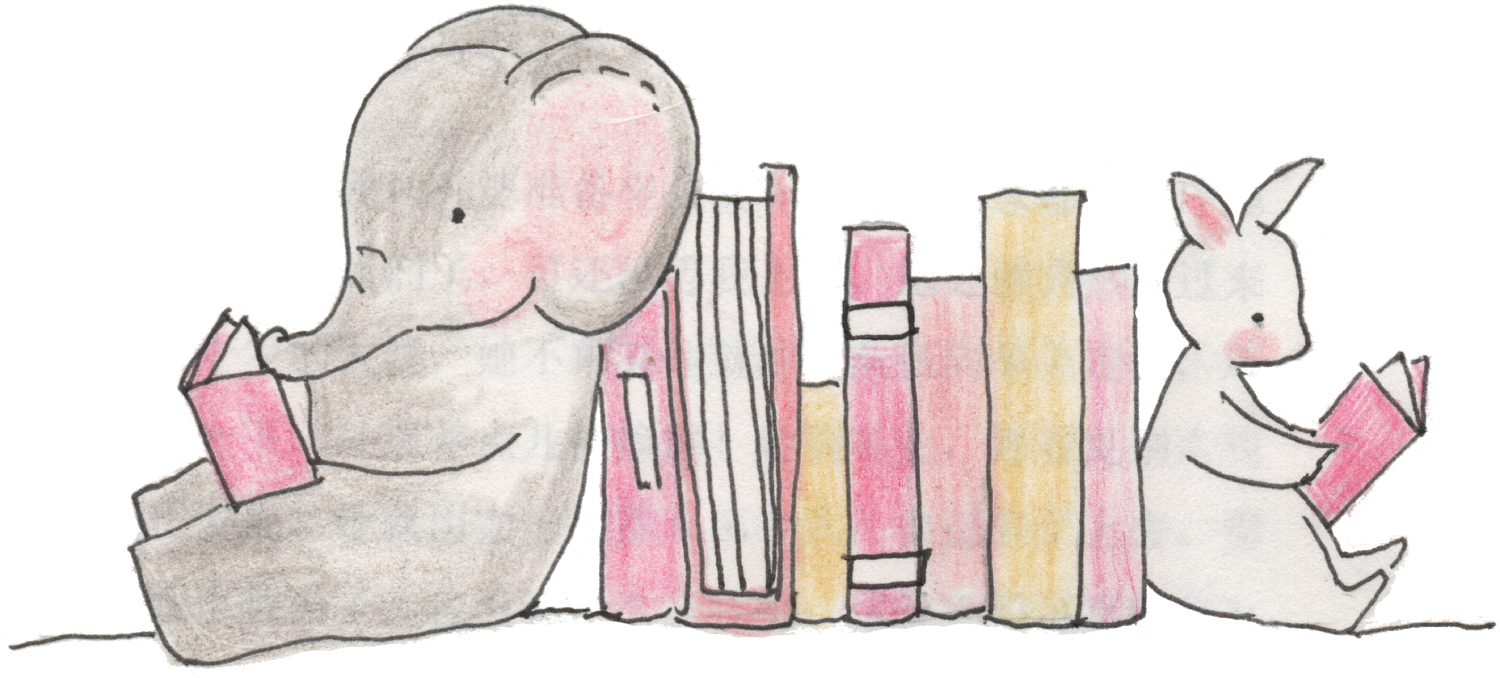
\includegraphics[width=\textwidth]{figure/02.png}
\end{figure}